\documentclass{beamer}

\usepackage[english]{babel}
\usepackage[utf8x]{inputenc}
\usepackage[T1]{fontenc}
\usepackage{lmodern}

%------ tikZ ------%
\usepackage{tikz}
\usetikzlibrary{positioning, arrows}
\usetikzlibrary{backgrounds}

%------------------%
\usepackage{ifthen}
\begin{document}

\begin{frame}[c]

\begin{center}
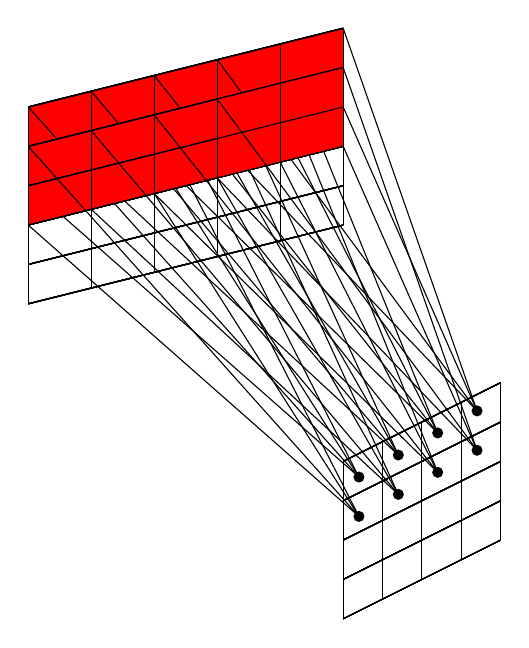
\begin{tikzpicture}
\pgfmathtruncatemacro\N{10}
\foreach \j in {1,...,8}{
    \onslide<\j>{
        \pgfmathsetmacro{\dx}{
            \j<5 ? (0.8*(\j-1)): (0.8*(\j-5))
            }
        \pgfmathsetmacro{\dy}{
            \j<5 ? (0.2*(\j-1)): (0.2*(\j-5)-0.5)
            }
        \pgfmathsetmacro{\tmp}{
            \j<5 ? (8) : (9)
        }
        %\begin{scope}[on background layer]
            \coordinate (a) at (0+\dx,3+\dy);
            \coordinate (d) at (0+\dx ,2+ \dy);
            \coordinate (b) at (1.6+\dx ,3.4+\dy);
            \coordinate (c) at (1.6+\dx,2.4+ \dy);
            \filldraw[fill=red,draw=none] (a) -- (b) -- (c) -- (d) --(a);
        %\end{scope}
        %\node[rectangle,draw] (r) at (\j,\j) {};

          \foreach \k in {1,...,6}
          {
          \pgfmathsetmacro{\idx}{0.2*(\k-1)}
          \pgfmathsetmacro{\sep}{0.8*(\k-1)}


          %horizontal lines
          \path[draw] (0,0.5*\k) -- (4,0.5*\k+1);
          %vertical lines
          \path[draw] (\sep,3+\idx) -- (\sep,0.5+\idx);

          }
          \foreach \k in {1,...,5}
          {
          \pgfmathsetmacro{\idx}{0.25*(\k-1)}
          \pgfmathsetmacro{\sep}{0.5*(\k-1)}


          %horizontal lines
          \path[draw] (4,0.5*\k-4) -- (6,0.5*\k+1-4);
          %vertical lines
          \path[draw] (4+\sep,-1.5+\idx) -- (4+\sep,-3.5+\idx);

          }
          \pgfmathsetmacro{\ccx}{
            \j<5 ? (4.2+0.5*(\j-1)): (4.2+0.5*(\j-5))
            }
            \pgfmathsetmacro{\ccy}{
                \j<5 ? (-1.7+0.28*(\j-1)): (-2.2+0.28*(\j-5))
                }
          \fill (\ccx,\ccy) circle (2pt);
          \path[draw] (a) -- (\ccx,\ccy);
          \path[draw] (b) -- (\ccx,\ccy);
          \path[draw] (c) -- (\ccx,\ccy);
          \path[draw] (d) -- (\ccx,\ccy);
    }
}
% \foreach \k in {1,...,\N}%
% {%
%     \pgfmathsetmacro\x{2.5*(\N-\k+1)/\N}
%     \onslide<\k>
%     {
%         \node[coordinate] at (0, 0) (bottomeLeft_corner) {};
%         \node[coordinate] at (\x, 1.25) (topRight_corner) {};
%         \path[fill=blue!20] (bottomeLeft_corner) rectangle (topRight_corner);
%         \node[above left=0.625cm and 2cm of bottomeLeft_corner, coordinate] (start1) {};
%         \node[above left=0.625cm and 0cm of bottomeLeft_corner, coordinate] (end1) {};
%         \draw[semithick] (start1) -- (end1);
%         \node[above right=-0.625cm and 0cm of topRight_corner, coordinate] (start2) {};
%         \node[above right=0.625cm and 4.5cm of bottomeLeft_corner, coordinate] (end2) {};
%         \draw[->, >=stealth', semithick] (start2) -- (end2);
%         \draw[semithick, black!40] (end1) -- (start2);
%         \node[below=0cm of end2, xshift=0.25cm] {time}; 
%         \node[yshift=-0.25cm] at (bottomeLeft_corner) {$t$};
%     }
% }
\end{tikzpicture}
\end{center}

\end{frame}

\end{document}